%Copyright 2014 Jean-Philippe Eisenbarth
%This program is free software: you can 
%redistribute it and/or modify it under the terms of the GNU General Public 
%License as published by the Free Software Foundation, either version 3 of the 
%License, or (at your option) any later version.
%This program is distributed in the hope that it will be useful,but WITHOUT ANY 
%WARRANTY; without even the implied warranty of MERCHANTABILITY or FITNESS FOR A 
%PARTICULAR PURPOSE. See the GNU General Public License for more details.
%You should have received a copy of the GNU General Public License along with 
%this program.  If not, see <http://www.gnu.org/licenses/>.

%Based on the code of Yiannis Lazarides
%http://tex.stackexchange.com/questions/42602/software-requirements-specification-with-latex
%http://tex.stackexchange.com/users/963/yiannis-lazarides
%Also based on the template of Karl E. Wiegers
%http://www.se.rit.edu/~emad/teaching/slides/srs_template_sep14.pdf
%http://karlwiegers.com
\documentclass{scrreprt}
\usepackage{listings}
\usepackage{underscore}
\usepackage[bookmarks=true]{hyperref}
\usepackage[utf8]{inputenc}
\usepackage[english]{babel}
\usepackage{CJKutf8}
\usepackage{graphicx}
\hypersetup{
    bookmarks=false,    % show bookmarks bar?
    pdftitle={Software Requirement Specification},    % title
    pdfauthor={Jean-Philippe Eisenbarth},                     % author
    pdfsubject={TeX and LaTeX},                        % subject of the document
    pdfkeywords={TeX, LaTeX, graphics, images}, % list of keywords
    colorlinks=true,       % false: boxed links; true: colored links
    linkcolor=blue,       % color of internal links
    citecolor=black,       % color of links to bibliography
    filecolor=black,        % color of file links
    urlcolor=purple,        % color of external links
    linktoc=page            % only page is linked
}%
\def\myversion{1.0 }
\date{}
%\title
\usepackage{hyperref}
\usepackage{pgf-umlcd}
\begin{document}

\begin{flushright}
    \rule{16cm}{5pt}\vskip1cm
    \begin{bfseries}
        \Huge{SOFTWARE REQUIREMENTS\\ SPECIFICATION}\\
        \vspace{1.5cm}
        for\\
       \vspace{1.5cm}
        FunMusic\\
       \vspace{1.5cm}
        \LARGE{Version \myversion approved}\\
        \vspace{1.5cm}
        \begin{CJK}{UTF8}{<font>}
        Prepared by 1040914 羅皓煒\\
        1041509 吳泰德\\
        1041513 白恬安\\
        1041514 張皓儒\\ 
        1043355 劉泳儀\\
        \end{CJK}
       \vspace{1.5cm}
       \begin{CJK}{UTF8}{<font>}
       元智大學 - 開放平台軟體課程\\
        \end{CJK}
        \vspace{1.3cm}
        \today
    \end{bfseries}
\end{flushright}

\tableofcontents


\chapter*{Revision History}

\begin{center}
    \begin{tabular}{|c|c|c|c|}
        \hline
	    Name & Date & Reason For Changes & Version\\
        \hline
	    Cindy & 06/28 & wrote five sections & 1\\
        \hline
	    4 & 32 & 33 & 34\\
        \hline
    \end{tabular}
\end{center}
%在center前後加上引入中文字需要的標籤後->依舊不可以打中文字,不知道為甚麼
%---------------------------------------------實作內容---------------------------------------------
%白恬安Cindy : 填寫三個Section的文字+確定中文字的運作
%------------------------------------------------------------------------------------------------------

\chapter{Introduction}

\section{Purpose}
\begin{CJK}{UTF8}{<font>}
        藉Line Bot系統實現根據使用者回傳的對話內容關鍵字,判斷使用者當下心情,並回傳相應的心情歌曲給使用者。希望透過與我們的Line Bot可以以音樂去安慰不開心的人,同時也可以讓開心的有更好的心情。另外藉由對話中出現的歌手名稱,可隨機推薦該歌手的影片MV連結。這是此程式的第一個版本,可以自己運作的主程式,而不是其他程式的部分元件。
%$<$Identify the product whose software requirements are specified in this  document指出即將被書寫在這份軟體說明書的產品是甚麼, including the revision or release number與其更改或釋出版本. Describe the scope of the product that is covered by this SRS, particularly if this SRS describes only part of the system or a single subsystem.說明這個產品的範圍。他是獨立的系統還是某個系統的部分元件$
\end{CJK}

\section{Document Conventions}
\begin{CJK}{UTF8}{<font>}
 本文以黑色粗體字表多個大小標題來做強調。
\end{CJK}

\section{Intended Audience and Reading Suggestions}
\begin{CJK}{UTF8}{<font>}
此份文件主要是給開發人員、產品經理人、以及未來的維護人員當作軟體開發時的參考依
據用的,不論是產品的需求、架構、效能......等都包含在此文件內,建議觀看方式為從
頭看到尾。若閱讀者為測試人員,須了解此程式能接收的輸入,以及此程式的需求,則可
以參考Product Functions、User Classes and Characteristics、Business Rules
以及User Documentati等部分。若閱讀者是使用者的話,可以直接參考User Documentation
的部分。
\end{CJK}

\section{Project Scope}
\begin{CJK}{UTF8}{<font>}
        使用的軟件分別是Microsoft Azure和Line Bot。
Microsoft Azure 中的文字分析的功用是可以對輸入文字進行情緒分析,
這API會為這句文字計算出一個心情數值由0到1之間,愈小表示心情愈不好,相反愈大表示愈開心。
而Line Bot是Line提供的API,可以與機器人進行構通。
為了達到產品可用音樂改善使用者的心情的這目的,而結合這兩項軟件。
任何人在任何時間都可以利用Line Bot去傳信息給機械人並把收到的文字用Azure的文字分析得到使用者心情
再從歌單中選出音樂推薦傳送給使用者。
%$<$Provide a short description of the software being specified and its purpose, including relevant benefits, objectives, and goals. Relate the software to corporate goals or business strategies. If a separate vision and scope document is available, refer to it rather than duplicating its contents here.$>$
\end{CJK}

\section{References}
\begin{CJK}{UTF8}{<font>}
% \begin{enumerate} \end{enumerate} 用來條列東西, 一個\item是一項
% \textbf用來弄粗體字
% \newline換行
\begin{enumerate} 
	\item \textbf {LINE developers} \newline
	https://developers.line.me/console/channel/1587699018/basic/
	\item  \textbf {Heroku} \newline
	https://dashboard.heroku.com
	\item \textbf {LineBot+Python,輕鬆建立聊天機器人} \newline
	https://yaoandy107.github.io/line-bot-tutorial/  
	\item  \textbf {文字分析API | Microsoft Azure}  \newline
	https://azure.microsoft.com/zh-tw/services/cognitive-services/text-analytics/
	\item  \textbf { LINE BOT 通訊}  \newline
	https://engineering.linecorp.com/tw/blog/detail/183
\end{enumerate}
%$<$List any other documents or Web addresses to which this SRS refers. These may  include user interface style guides, contracts, standards, system requirements specifications, use case documents, or a vision and scope document. Provide enough information so that the reader could access a copy of each reference, including title, author, version number, date, and source or location.$>$
\end{CJK}


\chapter{Overall Description}

\section{Product Perspective}
\begin{CJK}{UTF8}{<font>}
\textbf {\LARGE 這部分還沒弄Diagram圖表} \newline
在

$<$Describe the context and origin of the product being specified in this SRS.  
For example, state whether this product is a follow-on member of a product 
family, a replacement for certain existing systems, or a new, self-contained 
product. If the SRS defines a component of a larger system, relate the 
requirements of the larger system to the functionality of this software and 
identify interfaces between the two. A simple diagram that shows the major 
components of the overall system, subsystem interconnections, and external 
interfaces can be helpful.$>$
\end{CJK}

\section{Product Functions}
\begin{CJK}{UTF8}{<font>}

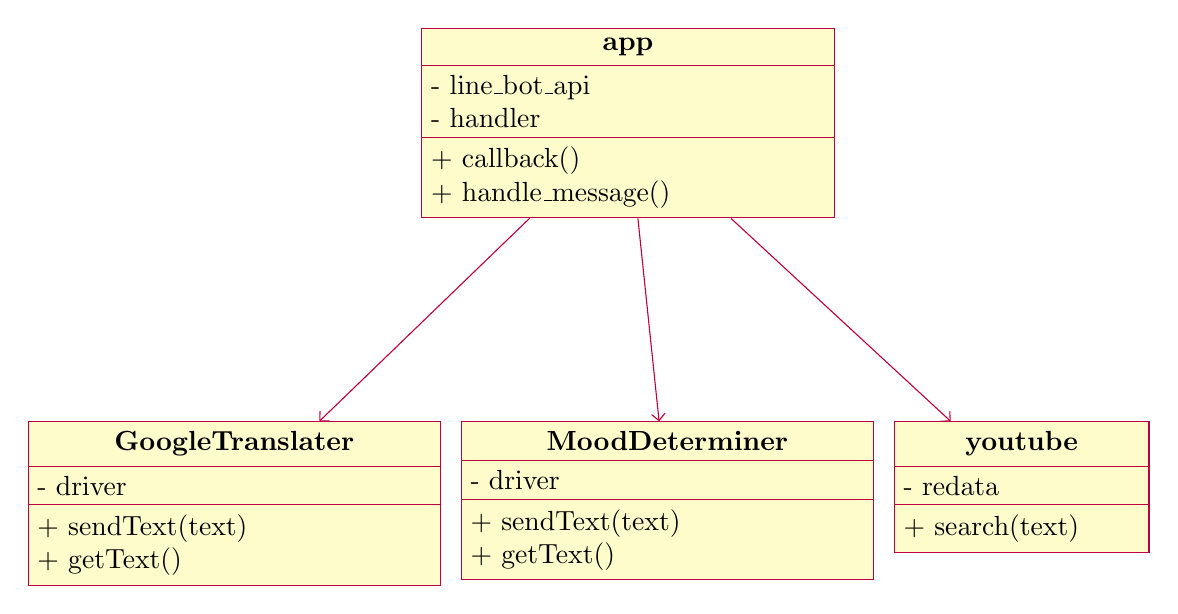
\begin{tikzpicture}% [ show background grid ]
\begin{class}[text width=3cm]{youtube}{5 ,-5}
\attribute{- redata}
\operation{+ search(text)}
\end{class}

\begin{class}[text width=5cm]{MoodDeterminer}{0.5 ,-5}
\attribute{- driver }
\operation{+ sendText(text)}
\operation{+ getText()}
\end{class}

\begin{class}[text width=5cm]{GoogleTranslater}{-5 ,-5}
\attribute{- driver }
\operation{+ sendText(text)}
\operation{+ getText()}
\end{class}

\begin{class}[text width=5cm]{app}{0 ,0}
\attribute{- line_bot_api}
\attribute{- handler}
\operation{+ callback()}
\operation{+ handle_message()}
\end{class}

\unidirectionalAssociation{app}{}{}{MoodDeterminer}
\unidirectionalAssociation{app}{}{}{GoogleTranslater}
\unidirectionalAssociation{app}{}{}{youtube}
\end{tikzpicture}

\end{CJK}

\section{User Classes and Characteristics}
\begin{CJK}{UTF8}{<font>}
本line bot預期的主要用戶為18到34歲的年輕人、line的中文用戶,因此本line bot推薦的音樂主要
為中文及英文的流行歌曲,並且在輸入方面也要求中文輸入。
\end{CJK}

\section{Operating Environment}
\begin{CJK}{UTF8}{<font>}
這個程式因為連結了line developer的後台系統,依賴著line現有的應用程式進行bot的實作。因此這個程式僅可以在支持line系統安裝的裝置上運作。目前智慧型手機主要使用的兩大作業系統,Android與IOS均有支持line系統的安裝。這個程式本身會回傳的語言為中文。只要裝置能安裝支持line bot系統使用的line應用程式,並能正常顯示繁體中文字,就可以正常使用本程式。
%$<$Describe the environment in which the software will operate程式的環境, including the hardware platform硬體平台, operating system and versions作業系統與版本, and any other software 
%components軟體元件 or applications應用 with which it must peacefully coexist或是不能與其相衝的程式.$>$
\end{CJK}

\section{Design and Implementation Constraints}
\begin{CJK}{UTF8}{<font>}
本程式伺服器架設於Heroku上,連結著line的bot系統運作。伺服器架設網站可以選擇其他網頁做使用。但因為對應於line系統介面與系統的設計,若轉換到其他bot系統使用,高機率會遇上函數不支持與版面設計不如預期等情況。
%$<$Describe any items or issues that will limit the options available to the developers. These might include: corporate or regulatory policies; hardware  limitations (timing requirements, memory requirements); interfaces to other applications; specific technologies, tools, and databases to be used; parallel operations; language requirements; communications protocols; security considerations; design conventions or programming standards (for example, if the customer’s organization will be responsible for maintaining the delivered software).$>$
\end{CJK}

\section{User Documentation}
\begin{CJK}{UTF8}{<font>}
本程式並無使用手冊或是線上引導的連結做提供。
%$<$List the user documentation components (such as user manuals, on-line help,  and tutorials) that will be delivered along with the software. Identify any known user documentation delivery formats or standards.$>$
\end{CJK}

\section{Assumptions and Dependencies}
\begin{CJK}{UTF8}{<font>}
本程式依賴line bot系統運作。雖然line為廣泛用於行動裝置的程式,但在已經確認行動裝置可以正常安裝與使用line的情況下,仍需注意該版本的line是否支持line bot的使用。line bot為近年新增的功能,不排除有過舊但仍可正常進行對話的line應用程式版本卻不支持使用line bot的可能性。
%$<$List any assumed factors (as opposed to known facts) that could affect the requirements stated in the SRS. These could include third-party or commercial components that you plan to use, issues around the development or operating environment, or constraints. The project could be affected if these assumptions are incorrect, are not shared, or change. Also identify any dependencies the project has on external factors, such as software components that you intend to reuse from another project, unless they are already documented elsewhere (for example, in the vision and scope document or the project plan).$>$
\end{CJK}

\chapter{External Interface Requirements}

\section{User Interfaces}
\begin{CJK}{UTF8}{<font>}
FunMusic是為所有人服務的一個設計,讓使用者可以在音樂中得到安慰和喜樂感。
主畫面是聊天的介面,一開始先輸入讓它啟動,然後屏幕會出現一個可按式表單。
可以點選來知道FunMusic的功能:搜歌模式和心情模式的操作說明。
還有,關於我們以及第四列的按鍵可以根據文字分析來推薦合適的音樂。
而當使用者用FunMusic搜歌模式時音樂可以用橫向滑動選擇。
\end{CJK}

\section{Hardware Interfaces}
\begin{CJK}{UTF8}{<font>}
本程式可在任何能實裝line的系統上運作,在輸入時需用到鍵盤,而在歌曲推薦時使用的
版面配置需用到左滑及右滑的功能,因此建議在手機或是平板等裝置上使用本程式。
\end{CJK}

\section{Software Interfaces}
\begin{CJK}{UTF8}{<font>}
$<$Describe the connections between this product and other specific software 
components (name and version), including databases, operating systems, tools, 
libraries, and integrated commercial components. Identify the data items or 
messages coming into the system and going out and describe the purpose of each.  
Describe the services needed and the nature of communications. Refer to 
documents that describe detailed application programming interface protocols.  
Identify data that will be shared across software components. If the data 
sharing mechanism must be implemented in a specific way (for example, use of a 
global data area in a multitasking operating system), specify this as an 
implementation constraint.$>$
\end{CJK}

\section{Communications Interfaces}
\begin{CJK}{UTF8}{<font>}
User使用Line Bot前端介面輸入訊息後,Line平台為了通訊的安全問題,資料都要會透過加密通道。
所以在架Messaging API的Webhook時,一定是用HTTPS來進行通訊協定。
而訊息傳出後經過根據Webhook URL(即Heroku的domain位置),通過Message API把訊息導到後端Heroku處理,
用HTTPS傳回到Message API,Heroku會根據Line Bot的Channel secret及Channel access token兩個key知道是哪個Line Bot
最後把訊息再發到平台上回覆使用者。[5]
\end{CJK}


\chapter{System Features}
\begin{CJK}{UTF8}{<font>}
$<$This template illustrates organizing the functional requirements for the 
product by system features, the major services provided by the product. You may 
prefer to organize this section by use case, mode of operation, user class, 
object class, functional hierarchy, or combinations of these, whatever makes the 
most logical sense for your product.$>$
\end{CJK}

\section{System Feature 1}
$<$Don’t really say “System Feature 1.” State the feature name in just a few 
words.$>$

\subsection{Description and Priority}
\begin{CJK}{UTF8}{<font>}
$<$Provide a short description of the feature and indicate whether it is of 
High, Medium, or Low priority. You could also include specific priority 
component ratings, such as benefit, penalty, cost, and risk (each rated on a 
relative scale from a low of 1 to a high of 9).$>$
\end{CJK}

\subsection{Stimulus/Response Sequences}
\begin{CJK}{UTF8}{<font>}
$<$List the sequences of user actions and system responses that stimulate the 
behavior defined for this feature. These will correspond to the dialog elements 
associated with use cases.$>$
\end{CJK}

\subsection{Functional Requirements}
\begin{CJK}{UTF8}{<font>}
$<$Itemize the detailed functional requirements associated with this feature.  
These are the software capabilities that must be present in order for the user 
to carry out the services provided by the feature, or to execute the use case.  
Include how the product should respond to anticipated error conditions or 
invalid inputs. Requirements should be concise, complete, unambiguous, 
verifiable, and necessary. Use “TBD” as a placeholder to indicate when necessary 
information is not yet available.$>$
\end{CJK}

$<$Each requirement should be uniquely identified with a sequence number or a 
meaningful tag of some kind.$>$

REQ-1:	REQ-2:

\section{System Feature 2 (and so on)}


\chapter{Other Nonfunctional Requirements}

\section{Performance Requirements}
\begin{CJK}{UTF8}{<font>}
由於本程式的伺服器建置在heroku的免費平台上,因此,倘若在30分鐘以內皆無使
用者對此程式進行輸入,則伺服器會自動關機,並在下一次接收到輸入時才重新啟動,所
以使用者第一次輸入時可能會有5~10秒的延遲時間。另外,因本程式在伺服器端主要運算
皆仰賴於爬蟲,所以如果同始有多位使用者進行輸入會造成伺服器頻繁的向目標網站送出
請求,可能會導致伺服器產生錯誤,無法正確回應使用者。
\end{CJK}

\section{Safety Requirements}
\begin{CJK}{UTF8}{<font>}
本程式為依賴著line bot系統的一個互動程式。因為系統主要擷取使用者對話判斷其心情並做進一步處理,因此line
系統本身擁有的「拍照並傳送圖片」、「傳送圖片」、「錄製語音並傳送」、「傳送貼圖」等等其他功能,使用者
雖然可以正常發送,但本程式撰寫出來的bot系統無法對其內容做出處理。僅會從預寫的文字訊息中隨機回覆一句,告知使用者已收到訊息,但無法處理。
%$<$Specify those requirements that are concerned with possible loss, damage, or  harm that could result from the use of the product. Define any safeguards or  actions that must be taken, as well as actions that must be prevented. Refer to  any external policies or regulations that state safety issues that affect the product’s design or use. Define any safety certifications that must be satisfied.$>$
\end{CJK}

\section{Security Requirements}
\begin{CJK}{UTF8}{<font>}
本程式程式本體儲存在Heroku,藉由Heroku系統將文字傳給line系統,因此文字訊息內容的安全性主要依賴line系統本身的加密系統。並不需要額外的加密系統。
%$<$Specify any requirements regarding security or privacy issues surrounding use of the product or protection of the data used or created by the product. Define any user identity authentication requirements. Refer to any external policies or  regulations containing security issues that affect the product. Define any  security or privacy certifications that must be satisfied.$>$
\end{CJK}

\section{Software Quality Attributes}
\begin{CJK}{UTF8}{<font>}
    \begin{enumerate} 
    \item \textbf {Reliability 可靠性} \newline
    本程式所使用的心情辨識以及翻譯系統皆仰賴於爬取外部網站的資料,且伺服器建置於
    heroku的免費平台上,因此本程式輸出的正確性皆由外部網站決定,並且隨著使用者的增
    加,伺服器也會更頻繁地向目標網站送出請求,從而導致可靠性也跟著降低。
    \item \textbf {Availability 可行性} \newline
    本程式的僅需做爬取特定網頁的資料以及部屬伺服器,因此可行性極高。
    \item \textbf {Portability 可移植性} \newline
    本程式主要建立在line的平台上,因此需用到line本身提供的api,若要移植本程式,需
    在額外撰寫別的聊天平台所提供的api。
    \end{enumerate}
\end{CJK}

\section{Business Rules}
\begin{CJK}{UTF8}{<font>}
若使用者告訴line bot想聽某歌手的音樂,則line bot會幫使用者找幾首該歌手的音樂,
若使用者只是單純地想與line bot抒發心情,則line bot會依照使用者語氣地不同而推薦
不同的歌曲。
\end{CJK}


\chapter{Other Requirements}
\begin{CJK}{UTF8}{<font>}
$<$Define any other requirements not covered elsewhere in the SRS. This might 
include database requirements, internationalization requirements, legal 
requirements, reuse objectives for the project, and so on. Add any new sections 
that are pertinent to the project.$>$
\end{CJK}

\section{Appendix A: Glossary}
\begin{CJK}{UTF8}{<font>}
%see https://en.wikibooks.org/wiki/LaTeX/Glossary
HTTP : HyperText Transfer Protocol\\
BOT : Build–operate–transfer
%$<$Define all the terms necessary to properly interpret the SRS, including  acronyms縮寫 and abbreviations縮寫. You may wish to build a separate glossary that spans multiple projects or the entire organization, and just include terms specific to a single project in each SRS.$>$
\end{CJK}

\section{Appendix B: Analysis Models}
\begin{CJK}{UTF8}{<font>}
None.
\end{CJK}

\section{Appendix C: To Be Determined List}
\begin{CJK}{UTF8}{<font>}
None.
\end{CJK}

\end{document}
